\documentclass{jamris}
\usepackage{amsmath,amssymb,booktabs}

\Author*{Kaveh Hooshmandi}{k.hooshmandi@arakut.ac.ir}{}{Arak University of Technology}{}{}
\Title{Randomized Model Predictive Control for F1TENTH Racing: A Simulation Case Study}
\Keywords{autonomous racing, randomized model predictive control, F1TENTH, Pure Pursuit, simulation benchmark}
\Year{2026}
\Num{--}
\Volnum{Draft}
\FirstPage{1}
\DOI{Draft manuscript; DOI pending}

\begin{document}
\maketitle

\begin{Abstract}
Randomized model predictive control (RMPC) has been demonstrated on a full-scale autonomous race car. We examine a public CUDA-based F1TENTH implementation, its two archived Indianapolis Motor Speedway (IMS) runs, and a new local run on an original, simplified Yas-Marina-inspired circuit. We then compare the implementation with a matched Pure Pursuit steering baseline in 100 independent, seeded, synchronous simulation trials: 80 nominal trials across two maps and three RMPC sample counts, plus 20 trials with a low-grip sector. Both methods share the centerline, speed policy, steering limits and LiDAR pipeline. All 100 trials completed one lap. At 5,000 samples, RMPC had mean root-mean-square lateral offsets of 0.184~m on IMS and 0.269~m on the new circuit; Pure Pursuit obtained 0.042 and 0.056~m, respectively. Mean laps were 53.51 versus 49.83~s on IMS and 61.16 versus 58.92~s on the new circuit. RMPC's median synchronized solve-call duration was approximately 0.92~ms; the largest observed solve call was 5.72~ms. A low-grip sector increased mean lateral error for both controllers. These results characterize this specific simulator, speed policy and perturbation protocol; they do not establish general superiority or full-scale equivalence.
\end{Abstract}

\section{Introduction}
Autonomous racing couples path tracking, fast computation, and operation near physical constraints. Muraleedharan, Sim\~oes, and Pau demonstrated GPU-based RMPC on a full-scale race car and reported a 115.72~s autonomous lap at Yas Marina Circuit, compared with a 105.34~s human-driven lap \cite{muraleedharan2025racing}. Their controller samples input sequences in the frequency domain to reduce undesirable command oscillation. The full-scale experiment motivates a smaller, accessible simulation study; its vehicle model, actuators, circuit, and lap times must not be transferred directly to a F1TENTH car.

The public F1TENTH RMPC repository \cite{mulakaloori2026repo} integrates a CUDA solver with a ROS~2 simulator, a LiDAR-derived local occupancy grid, and the IMS centerline. F1TENTH provides an open simulation environment for evaluating autonomous racing controllers \cite{okelly2020f1tenth}. This paper documents the control pipeline, presents the repository's recorded clear-track and slalom evidence, adds a local circuit run with a raw ROS~2 bag, and reports a controlled comparison against Pure Pursuit. The need for common benchmarks and explicit control-frequency evaluation has also been emphasized in F1TENTH research \cite{evans2024benchmarks}. Figure~\ref{fig:architecture} is an original schematic derived from the control concepts in \cite{muraleedharan2025racing} and the actual F1TENTH code \cite{mulakaloori2026repo}; it does not reproduce a figure from the reference article.

\section{Simulation and Controller}
\subsection{Environment and Reference}
The repository uses ROS~2 Humble, \texttt{f1tenth\_gym\_ros}, and an NVIDIA GPU. The recorded benchmarks were reported for an RTX~3090 with a configured speed ceiling of 10.5~m/s \cite{mulakaloori2026repo}. The supplied IMS centerline stores map coordinates $(x_i,y_i)$ and nominal left and right widths. Figure~\ref{fig:track} shows the original simplified circuit used in the new local experiments. The controller subscribes to odometry and LiDAR scans and publishes Ackermann steering and speed commands. The local grid has 0.05~m cells and nominal dimensions of $6\times3$~m, according to the configuration file.

For a vehicle position $\mathbf p=(x,y)$ and its nearest centerline sample $\mathbf p_i$, let $\mathbf t_i$ be the local unit tangent and $\mathbf n_i=(-t_{iy},t_{ix})$ its normal. The reported lateral variable is approximately
\begin{equation}
 d=(\mathbf p-\mathbf p_i)^\mathsf{T}\mathbf n_i.\label{eq:d}
\end{equation}
Thus $d$ is a track-relative lateral coordinate. It is analogous to the lateral error $y_e$ used in the full-scale paper \cite{muraleedharan2025racing}; it is not the global map coordinate $y$. The evaluator uses the nearest discrete point and tangent to compute $d$, while the online controller uses a nearby waypoint and its stored heading. This difference can cause small numerical differences between plotted and internal offsets.

\begin{figure}[htb]
\centering
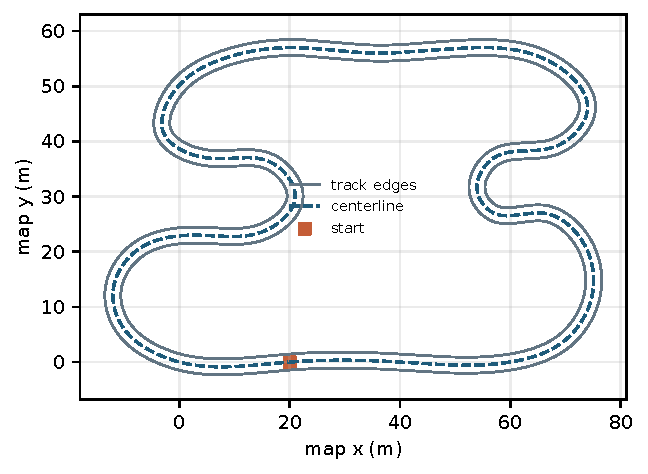
\includegraphics[width=\columnwidth]{figures/f1_track.pdf}
\caption{Original simplified Yas-Marina-inspired circuit used in the local experiments. The generated centerline, track edges, and start location share one map coordinate system; the nominal road width is 2.9~m.}
\label{fig:track}
\end{figure}

\subsection{Prediction and Actuation}
At each odometry callback, the implementation projects the vehicle state into Frenet coordinates $(s,d,e_\psi)$, builds a centerline horizon, and invokes the GPU randomized solver. The configured horizon contains 100 stages at $\Delta t=0.02$~s and 5,000 sampled rollouts, with seven basis coefficients. The nominal horizon is 2.0~s; the stored states at indices 0--99 span 99 transitions, or 1.98~s. A cost for track-relative error, actuation, stability, boundary violation, and occupancy-grid intersection ranks candidate steering sequences \cite{mulakaloori2026repo}. The solver returns a steering action; the published speed is computed separately. The full-scale paper optimizes steering, throttle, and brake inputs, while holding gear constant during prediction and handling gear changes with separate logic \cite{muraleedharan2025racing}.

The speed command uses a curvature ceiling of the form
\begin{equation}
 v_{\kappa}=\sqrt{\frac{\mu g}{\max_{k}|\kappa_k|+10^{-4}}},\label{eq:speed}
\end{equation}
where the code uses $\mu=0.523$ and bounds the final target to 2.5--10.5~m/s. A forward-obstacle-distance term also limits that target, followed by an acceleration and deceleration slew limiter. Equation~\ref{eq:speed} describes the implementation's heuristic speed ceiling; it is not an experimentally validated tire-grip limit. The LiDAR grid is inflated around observed cells, and predicted grid occupancy incurs a cost in the steering rollout. Figure~\ref{fig:architecture} summarizes the signal flow.

\begin{figure*}[t]
\centering
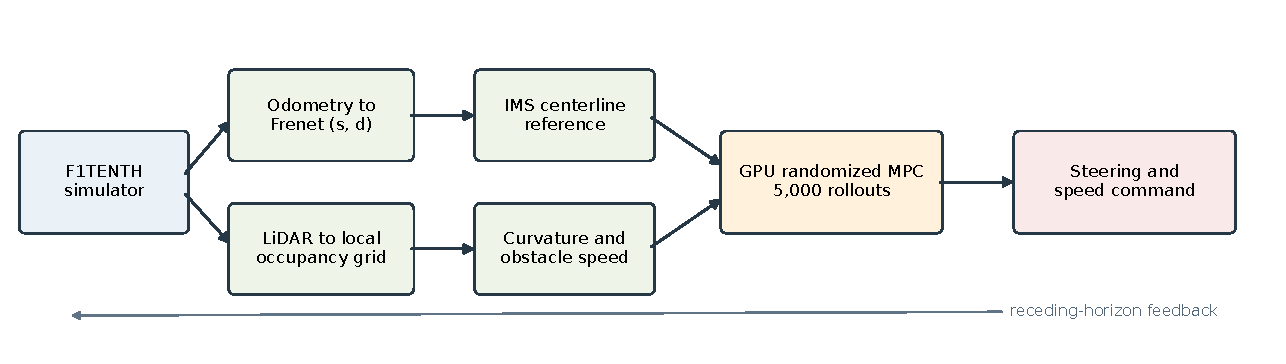
\includegraphics[width=.92\textwidth]{figures/architecture.pdf}
\caption{Original signal-flow schematic of the repository implementation. The GPU solver selects steering; a separate speed planner produces the speed command. The layout is informed by the RMPC controller description in \cite{muraleedharan2025racing} and verified against \cite{mulakaloori2026repo}.}
\label{fig:architecture}
\end{figure*}

% Technical development based on IV2025_arun.pdf and the pinned implementation.
\subsection{Dynamic Bicycle Model and Tire Forces}
The full-scale formulation in Sections~III--IV of \cite{muraleedharan2025racing} uses a dynamic bicycle model in a Frenet frame. Each axle represents the combined action of its two tires. Progress $s$, lateral offset $d$, heading error $e_\psi$, body-frame velocities $v_x,v_y$, and yaw rate $r$ describe motion. With path curvature $\kappa(s)$, steering angle $\delta$, mass $m$, yaw inertia $I_z$, and axle distances $l_f,l_r$, its motion equations can be written as
\begin{equation}
\begin{aligned}
\dot s &= \frac{v_x\cos e_\psi-v_y\sin e_\psi}{1-d\kappa},\\
\dot d &= v_x\sin e_\psi+v_y\cos e_\psi,\\
\dot e_\psi &= r-\kappa\dot s,\\
m\dot v_x &= F_{xr}-F_D-F_{yf}\sin\delta\\
 &\quad +F_{xf}\cos\delta+mv_yr,\\
m\dot v_y &= F_{yr}+F_{yf}\cos\delta\\
 &\quad +F_{xf}\sin\delta-mv_xr,\\
I_z\dot r &= l_f(F_{yf}\cos\delta+F_{xf}\sin\delta)\\
 &\quad -l_rF_{yr}.
\end{aligned}\label{eq:fullmodel}
\end{equation}
Here $F_{xi},F_{yi}$ denote longitudinal and lateral axle forces, and $F_D$ denotes aerodynamic drag. The reference article models engine force as a function of throttle, speed, and gear, and models brake force and rolling resistance separately. These powertrain terms belong to its full-scale vehicle model; they are not identified F1TENTH parameters.

The F1TENTH solver uses the reduced state $\mathbf x=[s,d,e_\psi,v_y,r]^\mathsf T$ and scalar input $u=\delta$ \cite{mulakaloori2026repo,muraleedharan2026solver}. The imported solver is pinned at revision \texttt{2c25f4b}. Its forward speed is held constant during each rollout at $\bar v_x=\max(2.5,v_x^{\rm odom})$. It retains the first three equations in Eq.~\ref{eq:fullmodel} and uses
\begin{equation}
\begin{aligned}
\dot v_y &= (F_{yf}\cos\delta+F_{yr})/m-\bar v_xr,\\
\dot r &= (l_fF_{yf}\cos\delta-l_rF_{yr})/I_z.
\end{aligned}\label{eq:reducedmodel}
\end{equation}
The code propagates these states by forward Euler integration, $\mathbf x_{k+1}=\mathbf x_k+\Delta t f(\mathbf x_k,\delta_k)$. Curvature and track widths come from the reference horizon, with desired lateral offset zero. Frenet coordinates require $1-d\kappa\ne0$; the model is intended for motion near the reference path.

Both formulations use a Pacejka-type nonlinear lateral-force law. For the F1TENTH implementation it is
\begin{equation}
\begin{aligned}
F_{yi}&=\mu F_{zi}\sin\!\left[C_i\arctan\!\left(z_i\right)\right],\\
z_i&=B_i\alpha_i-E_i\bigl(B_i\alpha_i-\arctan(B_i\alpha_i)\bigr),\\
\alpha_f&=\arctan\!\frac{v_y+l_fr}{v_{\rm slip}}-\delta,\\
\alpha_r&=\arctan\!\frac{v_y-l_rr}{v_{\rm slip}}.
\end{aligned}\label{eq:tire}
\end{equation}
For the configured zero aerodynamic lift coefficients, $F_{zf}=mg l_r/(l_f+l_r)$ and $F_{zr}=mg l_f/(l_f+l_r)$. Table~\ref{tab:configuration} lists the parameters used in the repository. The reference paper additionally identifies lateral-force offsets and refines its tire model with measured race-car data; those fitted full-scale values are not reused here.

An implementation detail affects Eq.~\ref{eq:tire}: the imported car-steering model uses $v_{\rm slip}=\max(7.0,\bar v_x)$ in m/s. Although the outer F1TENTH header declares a 0.5~m/s constant, it delegates dynamics to the imported model, whose 7.0~m/s floor is active. Thus slip predictions below 7~m/s use a larger denominator than the measured speed. This is a code property of the pinned revision, not a physical tire law, and should be reviewed when tuning low-speed behavior.

\begin{table}[htb]
\centering
\caption{F1TENTH settings from \texttt{config/config.yaml} in \cite{mulakaloori2026repo}. They are configuration values, not parameters measured in the full-scale paper.}
\label{tab:configuration}
\small
\begin{tabular}{lr}
\toprule
Parameter & Value\\
\midrule
Mass $m$ & 3.47 kg\\
Yaw inertia $I_z$ & 0.04712 kg\,m$^2$\\
Front/rear axle distance & 0.15875 / 0.17145 m\\
Wheelbase / body width & 0.3302 / 0.2032 m\\
Friction coefficient $\mu$ & 0.523\\
Front $(B,C,E)$ & $(-6,1.5,-0.1)$\\
Rear $(B,C,E)$ & $(-7,1.5,-0.1)$\\
Steering magnitude limit & 0.4189 rad\\
Steering rate limit & 3.2 rad/s\\
Speed range & 2.5--10.5 m/s\\
Acceleration/deceleration & 7.51 / 8.26 m/s$^2$\\
Stages / samples / basis modes & 100 / 5,000 / 7\\
Rollout step / initial seed & 0.02 s / 70997\\
Warm start & enabled\\
Grid inflation half-width & 4 cells (0.20 m)\\
\bottomrule
\end{tabular}
\end{table}

\subsection{Frequency-Domain Sampling and Input Constraints}
The reference article motivates IDCT sampling because independently sampled time-domain inputs can oscillate excessively \cite{muraleedharan2025racing}. Its algorithm combines steering and longitudinal-force samples before evaluating the vehicle response. The F1TENTH implementation instead evaluates 5,000 scalar steering sequences. The following explicit construction is taken from the imported solver code \cite{muraleedharan2026solver}, supplementing the conceptual description in the article.

Let $N=100$ and $M=7$. Its orthonormal cosine basis is
\begin{equation}
 b_{ki}=\sqrt{2/N}\,c_i\cos\!\left(\frac{\pi i(k+1/2)}{N}\right),
\end{equation}
where $c_0=1/\sqrt{2}$ and $c_i=1$ for $i>0$. For random candidate $j$, coefficients $a_{ij}$ are drawn uniformly in $(-1,1]$. With $h=\dot\delta_{\max}\Delta t$, the increments and bounded commands are
\begin{equation}
\begin{aligned}
\eta_k^{(j)} &=h\sum_{i=0}^{M-1}b_{ki}a_{ij},\\
\delta_k^{(j)} &=\operatorname{clip}_{[-\delta_{\max},\delta_{\max}]}\!\left(
\delta_{k-1}^{(j)}+\operatorname{clip}_{[-h,h]}\eta_k^{(j)}\right).
\end{aligned}\label{eq:idct}
\end{equation}
All candidates start with the current command at $k=0$. The configured rate limit gives $h=0.064$~rad per rollout step. Using low cosine modes restricts rapid variation before clipping. Candidate zero holds the current command; when available, candidate one reuses a shifted previous best sequence under the same limits. This preserves a warm-start candidate without implying global optimality.

\subsection{Tracking, Grip, and Obstacle Costs}
The full-scale article balances tracking error, command variation, terminal error, and tire-grip penalties. In compact notation, its objective has the form
\begin{equation}
\begin{aligned}
J_{\rm IV}={}&\sum_k\left(\mathbf e_k^\mathsf TQ\mathbf e_k+
\Delta\mathbf u_k^\mathsf TR\Delta\mathbf u_k\right)\\
&+\mathbf e_N^\mathsf TQ_f\mathbf e_N
 +\sum_{k,i}q_{g,i}P_{g,i}(k).
\end{aligned}\label{eq:ivcost}
\end{equation}
Here $\mathbf e_k$ denotes tracking error and $\Delta\mathbf u_k$ successive command changes. This notation summarizes Eq.~(11) of \cite{muraleedharan2025racing}. The reference study considers combined force $F_i=\sqrt{F_{xi}^2+F_{yi}^2}$ relative to $\mu_iF_{zi}$ and uses the smooth penalty
\begin{equation}
P_{g,i}=\log\!\left[1+e^{A(F_i/F_{zi}-\mu_{\rm lim})}\right]
-\log\!\left[1+e^{-A\mu_{\rm lim}}\right].
\end{equation}
It penalizes tire-force utilization near the chosen grip threshold. Actuator amplitude and rate bounds restrict sampled commands, whereas a finite grip penalty does not guarantee constraint satisfaction.

The actual F1TENTH cost differs from Eq.~\ref{eq:ivcost}. Define the error penalty $E(z;q,c,l)=\min(qz^2,c)+l|z|$. With $w_k=(1-0.3k/(N-1))/N$, the implementation evaluates
\begin{equation}
\begin{aligned}
J_{\rm F1}={}&\sum_{k=0}^{N-1}\left(w_kL_k+
\frac{20000}{N}\mathbb I_{\rm occ}(\mathbf x_k)\right)\\
&+\frac{E_{d,T}(d_{N-1})+E_{\psi,T}(e_{\psi,N-1})}{N},\\
L_k={}&E_d(d_k)+E_\psi(e_{\psi,k})+0.05\delta_k^2-0.5s_k\\
&+5(\delta_k-\delta_{k-1})^2
 +P_{f,k}+P_{r,k}+P_{b,k}+P_{\alpha,k}.
\end{aligned}\label{eq:f1cost}
\end{equation}
The command-change term is zero at $k=0$. The $(q,c,l)$ triples are $(400,600,50)$ for lateral error and $(3500,250,500)$ for heading error; terminal triples are $(200,400,20)$ and $(1500,200,100)$. The negative progress term rewards forward motion. The force penalties $P_f,P_r$ use lateral-force utilization $z_i=|F_{yi}|/(\mu F_{zi})$ and the barrier $2\{\log[1+\exp(20(z_i-1))]-\log[1+\exp(-20)]\}$. In particular, the configured pair \texttt{[20,2]} maps to sharpness 20 and multiplier 2 in the imported structure.

For each track side, $P_b$ adds a linear penalty of gain 1500 for exceeding the boundary after subtracting half the car width and an extra 0.08~m margin, capped at 1000 per side. The slip penalty adds $\min(5000,1000\max(0,|\alpha_i|-0.15))$ per axle. These terms express preferences through finite costs.

The occupancy indicator in Eq.~\ref{eq:f1cost} is obtained by projecting a predicted Frenet state into the local LiDAR grid, using curvature at the current vehicle position. A hit in an inflated occupied cell adds $20000/N=200$ per stage, independently of $w_k$. LiDAR returns are inflated by a square extending four cells in each direction. The lookup treats positions outside the local grid as unoccupied, so grid extent and the constant-curvature projection limit what this obstacle cost observes. The objective minimizes cost over the sampled candidates; it supplies neither a continuous-optimization optimum nor a formal collision-avoidance guarantee.

\subsection{Receding-Horizon Execution on the GPU}
The implementation follows the sampling, prediction, evaluation, and selection sequence of Algorithm~1 in \cite{muraleedharan2025racing}, specialized to steering:
\begin{enumerate}
\item Convert odometry to the five-state Frenet model and construct the reference horizon. Update the local grid from available LiDAR scans.
\item Generate bounded IDCT steering sequences, including the hold and warm-start candidates.
\item Propagate each candidate through Eqs.~\ref{eq:reducedmodel}--\ref{eq:tire} and accumulate Eq.~\ref{eq:f1cost}. CUDA executes candidate rollouts in parallel, with sequential state propagation within each candidate.
\item Copy candidate costs to the host and select the smallest finite cost. Copy the winning trajectory and retain it for the next warm start.
\item Publish the winning sequence's element at index 1, since index 0 is the current command. Compute the speed command separately and repeat at the next odometry callback.
\end{enumerate}
The node publishes zero speed and steering if the solver returns an error. The initial random seed is 70997 and is incremented by the solve-call index. Consequently, reproducing the sampled sequence also depends on the sequence of callbacks. Unlike a wholly GPU-resident minimum-cost reduction, this pinned solver selects the winner on the CPU after copying all candidate costs. This distinction matters when interpreting timing relative to the GPU-focused full-scale study.

The separate speed command uses Eq.~\ref{eq:speed}, a forward-grid-distance heuristic, and clipping to the configured speed range. Its slew limiter advances by $a_{\max}\Delta t$ or $b_{\max}\Delta t$ per callback using the configured rollout step, rather than measured callback spacing. Therefore the tabulated acceleration settings are nominal increments in that implementation; their realized per-second effect depends on the callback rate. The speed floor is not a stopping policy near obstacles. These details should be included when reproducing or modifying the controller.


\subsection{RViz Views from the Public Implementation}
The two RViz screenshots in Fig.~\ref{fig:rviz} are taken directly from the repository's \texttt{results/} directory \cite{mulakaloori2026repo}. Its README identifies the yellow dashed centerline, the white local occupancy-grid display, black inflated obstacle cells, cyan candidate rollouts, a red selected trajectory, and green detected obstacle cells. The left image provides an overview of the vehicle and local prediction region. The right image shows the obstacle-view screenshot: detected cells lie ahead of the vehicle while the selected trajectory passes to their left. These are visualizations of individual simulator states. They demonstrate how the map, LiDAR grid, and predicted path appear together, but they do not by themselves establish obstacle clearance or a lap-time result; those quantities come from the recorded evaluator output in Section~4.

\begin{figure*}[t]
\centering
\begin{minipage}[t]{.49\textwidth}
\centering
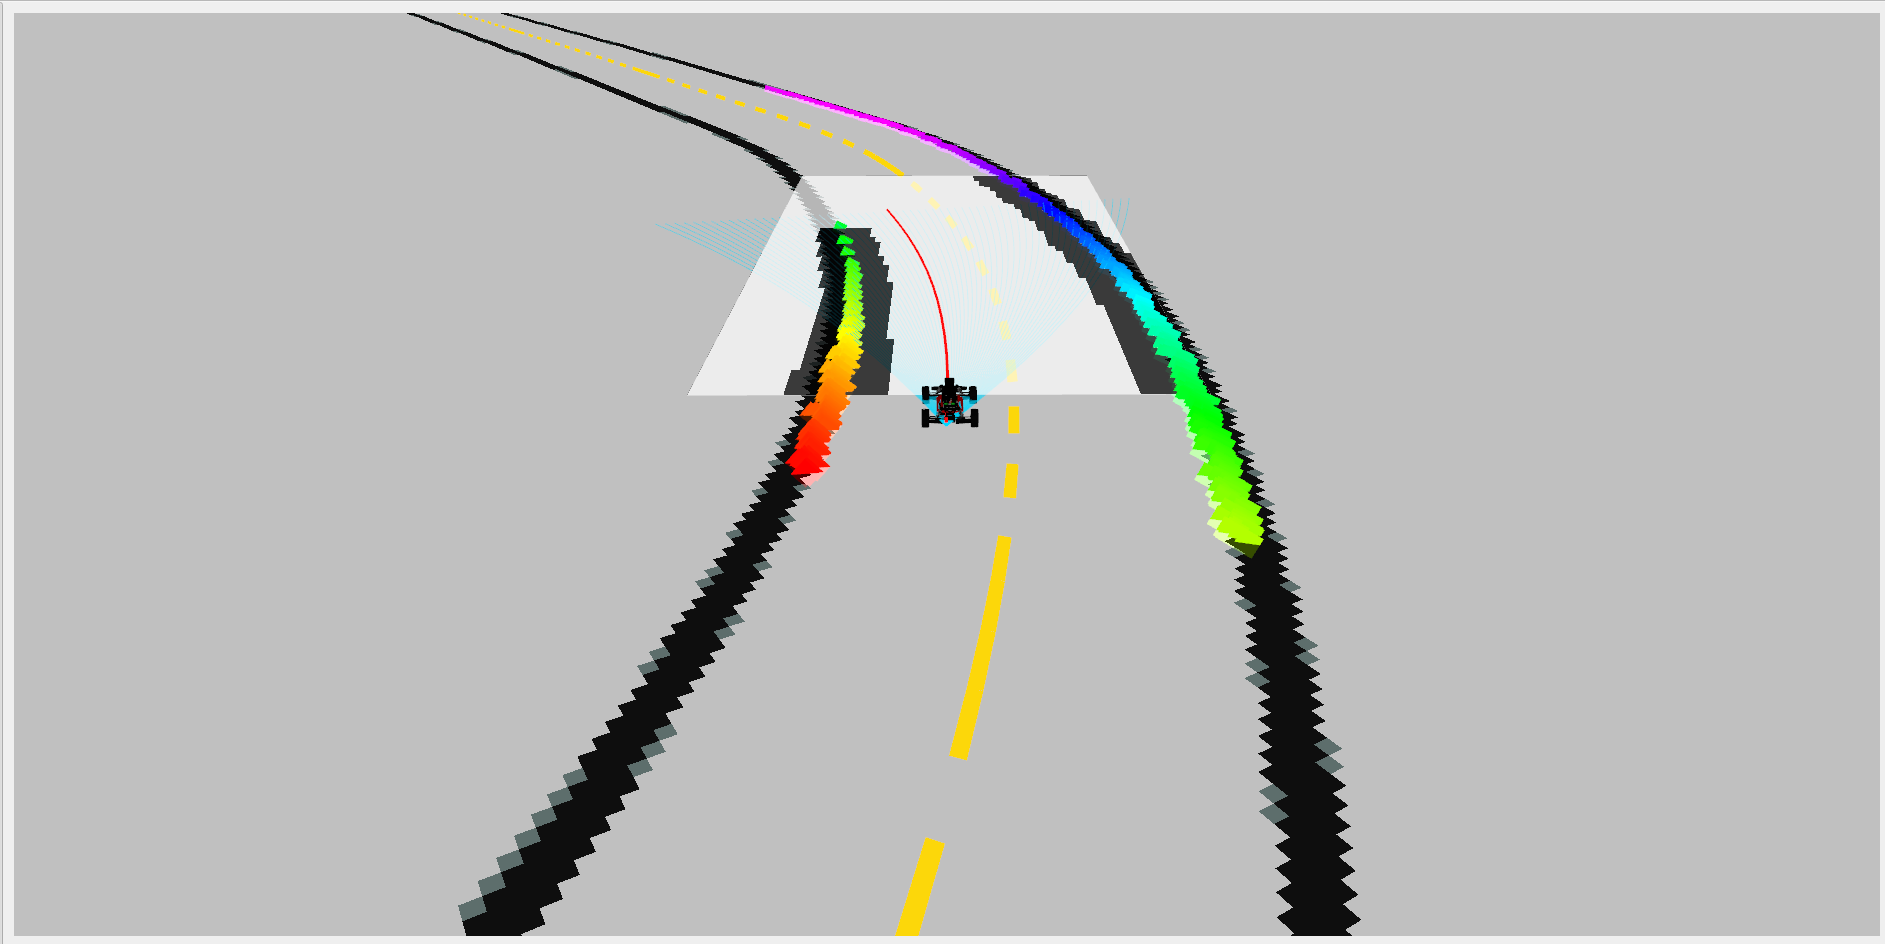
\includegraphics[width=\linewidth]{figures/rviz_screenshot.png}\\[-1mm]
\small (a) RViz overview
\end{minipage}\hfill
\begin{minipage}[t]{.49\textwidth}
\centering
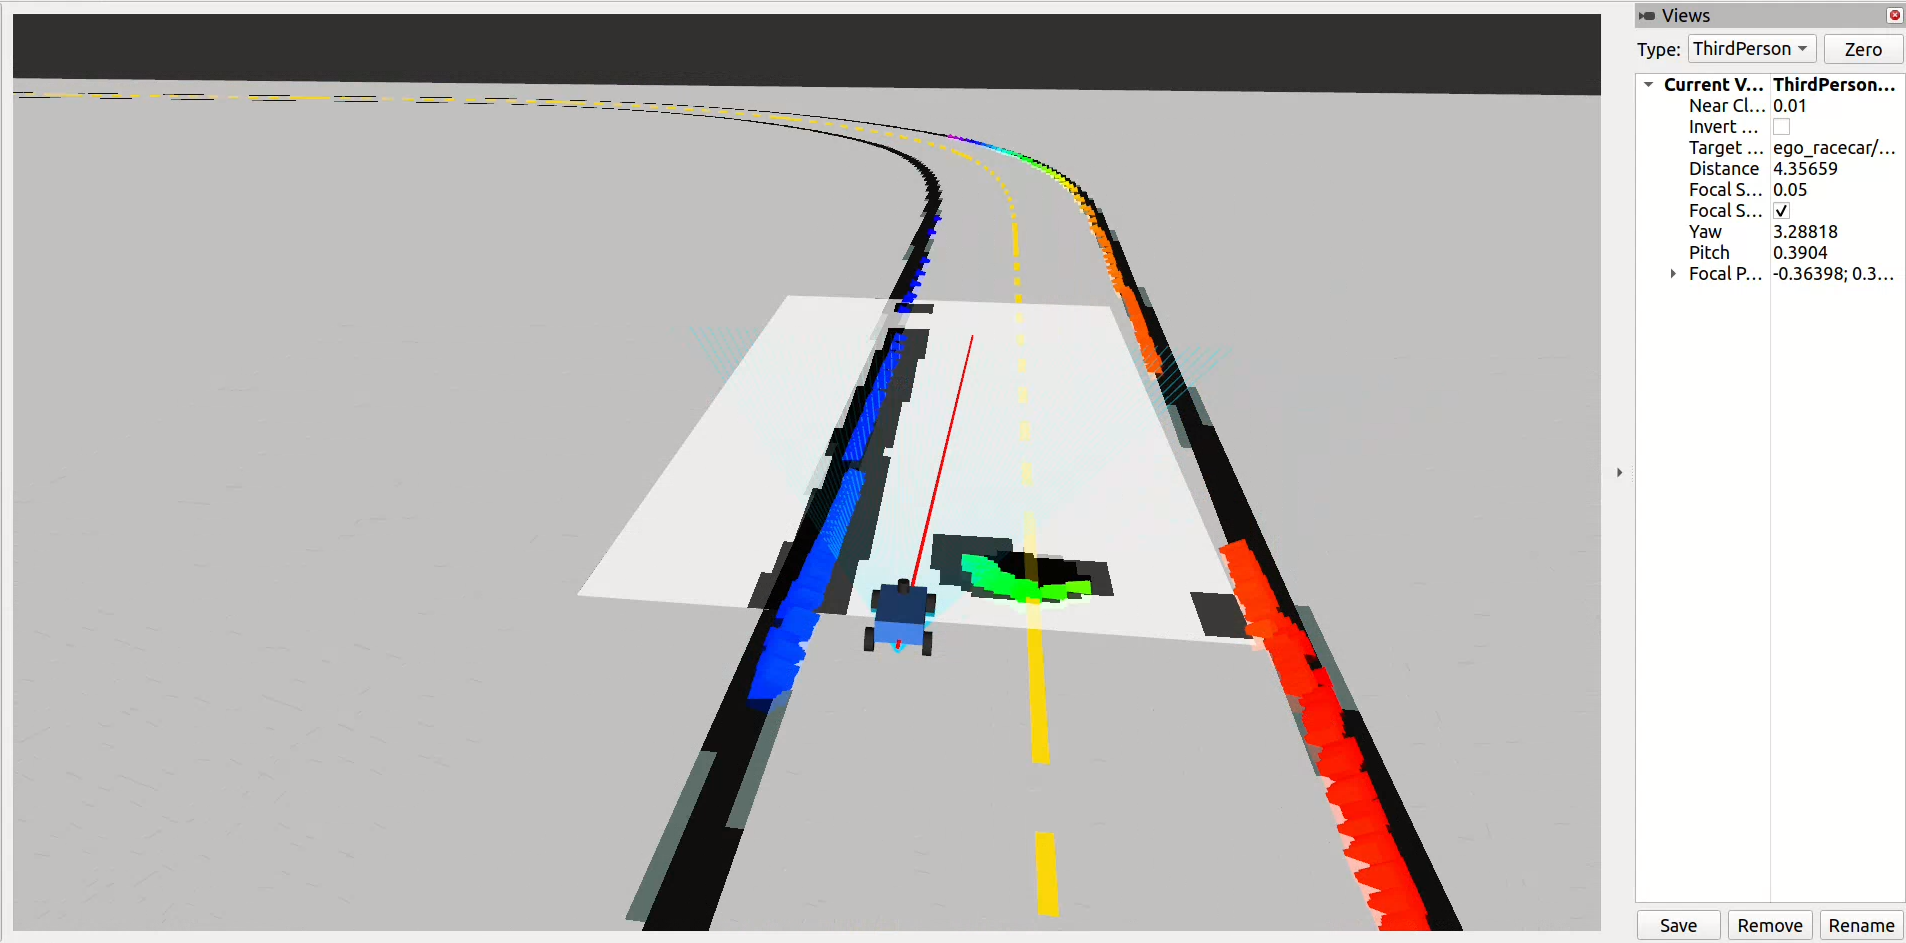
\includegraphics[width=\linewidth]{figures/rviz_obstacles_screenshot.png}\\[-1mm]
\small (b) RViz obstacle view
\end{minipage}
\caption{RViz views reproduced from \texttt{results/rviz\_screenshot.png} and \texttt{results/rviz\_obstacles\_screenshot.png} in the RMPC simulation repository \cite{mulakaloori2026repo} (Apache-2.0). The repository README supplies the display-color interpretation described in the text.}
\label{fig:rviz}
\end{figure*}

\section{Evaluation Method}
We treat the published JSON summaries and PNG plots in repository revision \texttt{c5c190f} as the source dataset \cite{mulakaloori2026repo}. The raw ROS~2 bags are not included in the repository, so the original trajectories and message-level statistics cannot be independently recomputed here. The two source cases are a nominal clear-track run and a run with three fixed obstacle points. Separately, we recorded a local ROS~2 bag on a new circuit using the same controller snapshot and evaluator. The evaluator detects laps when nearest-centerline progress wraps from above 90\% to below 10\% of track length. It estimates obstacle clearance by subtracting a 0.25~m obstacle radius and a 0.20~m vehicle radius from center-to-center distance. This is a point-and-circle geometric estimate, not a simulator contact check. In no-obstacle runs, the evaluator stores a 10,000~m placeholder rather than a measured clearance; therefore no clearance is reported for them.

The evaluator plots $d(t)$, nearest-obstacle gap, and commanded versus kinematically inferred steering. It also takes differences between consecutive \texttt{/drive} message timestamps. Because the solver runs in an odometry callback before publishing, these intervals include controller execution, ROS scheduling, and other overhead; they do not isolate GPU kernel time. The configured 20~ms rollout step is shown as a reference value, not proof of a measured 50~Hz deadline.

\section{Simulation Results}
Table~\ref{tab:results} transcribes the saved benchmark summaries. The clear-track run records two detected laps, 34.77 and 32.62~s, over 70.74~s of analyzed odometry. The slalom records one detected lap of 39.09~s over 43.12~s. The slalom fastest lap is 6.47~s longer than the clear-track fastest lap, a descriptive difference of 19.8\%. With only one slalom lap and no repeated trials, this is not an estimate of a general obstacle penalty.

\begin{table}[htb]
\centering
\caption{Repository-reported results from one clear-track and one slalom run. ``--'' means inapplicable or unavailable.}
\label{tab:results}
\small
\begin{tabular}{lrr}
\toprule
Metric & Clear track & Slalom\\
\midrule
Detected laps & 2 & 1\\
Fastest lap (s) & 32.62 & 39.09\\
Mean lap (s) & 33.69 & 39.09\\
Analyzed duration (s) & 70.74 & 43.12\\
Min. obstacle gap (m) & -- & 0.054\\
Mean drive interval (ms) & 7.37 & 7.03\\
P99 drive interval (ms) & 16.69 & 16.79\\
Max. drive interval (ms) & 19.91 & 335.87\\
\bottomrule
\end{tabular}
\end{table}

\subsection{Lateral $y$ Response and Obstacle Passage}
Figure~\ref{fig:yresponse} is the repository's recorded slalom plot. Its upper trace is the requested lateral $y$ simulation response, represented by $d(t)$ in Eq.~\ref{eq:d}. The trace changes sign as the vehicle follows the IMS route and passes obstacles. The middle trace shows four close-approach events in the displayed window and remains above zero; the JSON summary gives a minimum estimated gap of 0.054~m over the run. The lower trace shows the published steering command and a steering angle inferred by the evaluator from speed and yaw rate. The dashed $d=\pm4$~m lines in the source plot are plotting guides, not the IMS track boundaries; the source CSV gives nominal 1.1~m widths on each side. The plot supports qualitative lateral-response and obstacle-passage observations, but it does not provide raw samples for exact RMS tracking error or a verified collision rate.

\begin{figure*}[t]
\centering
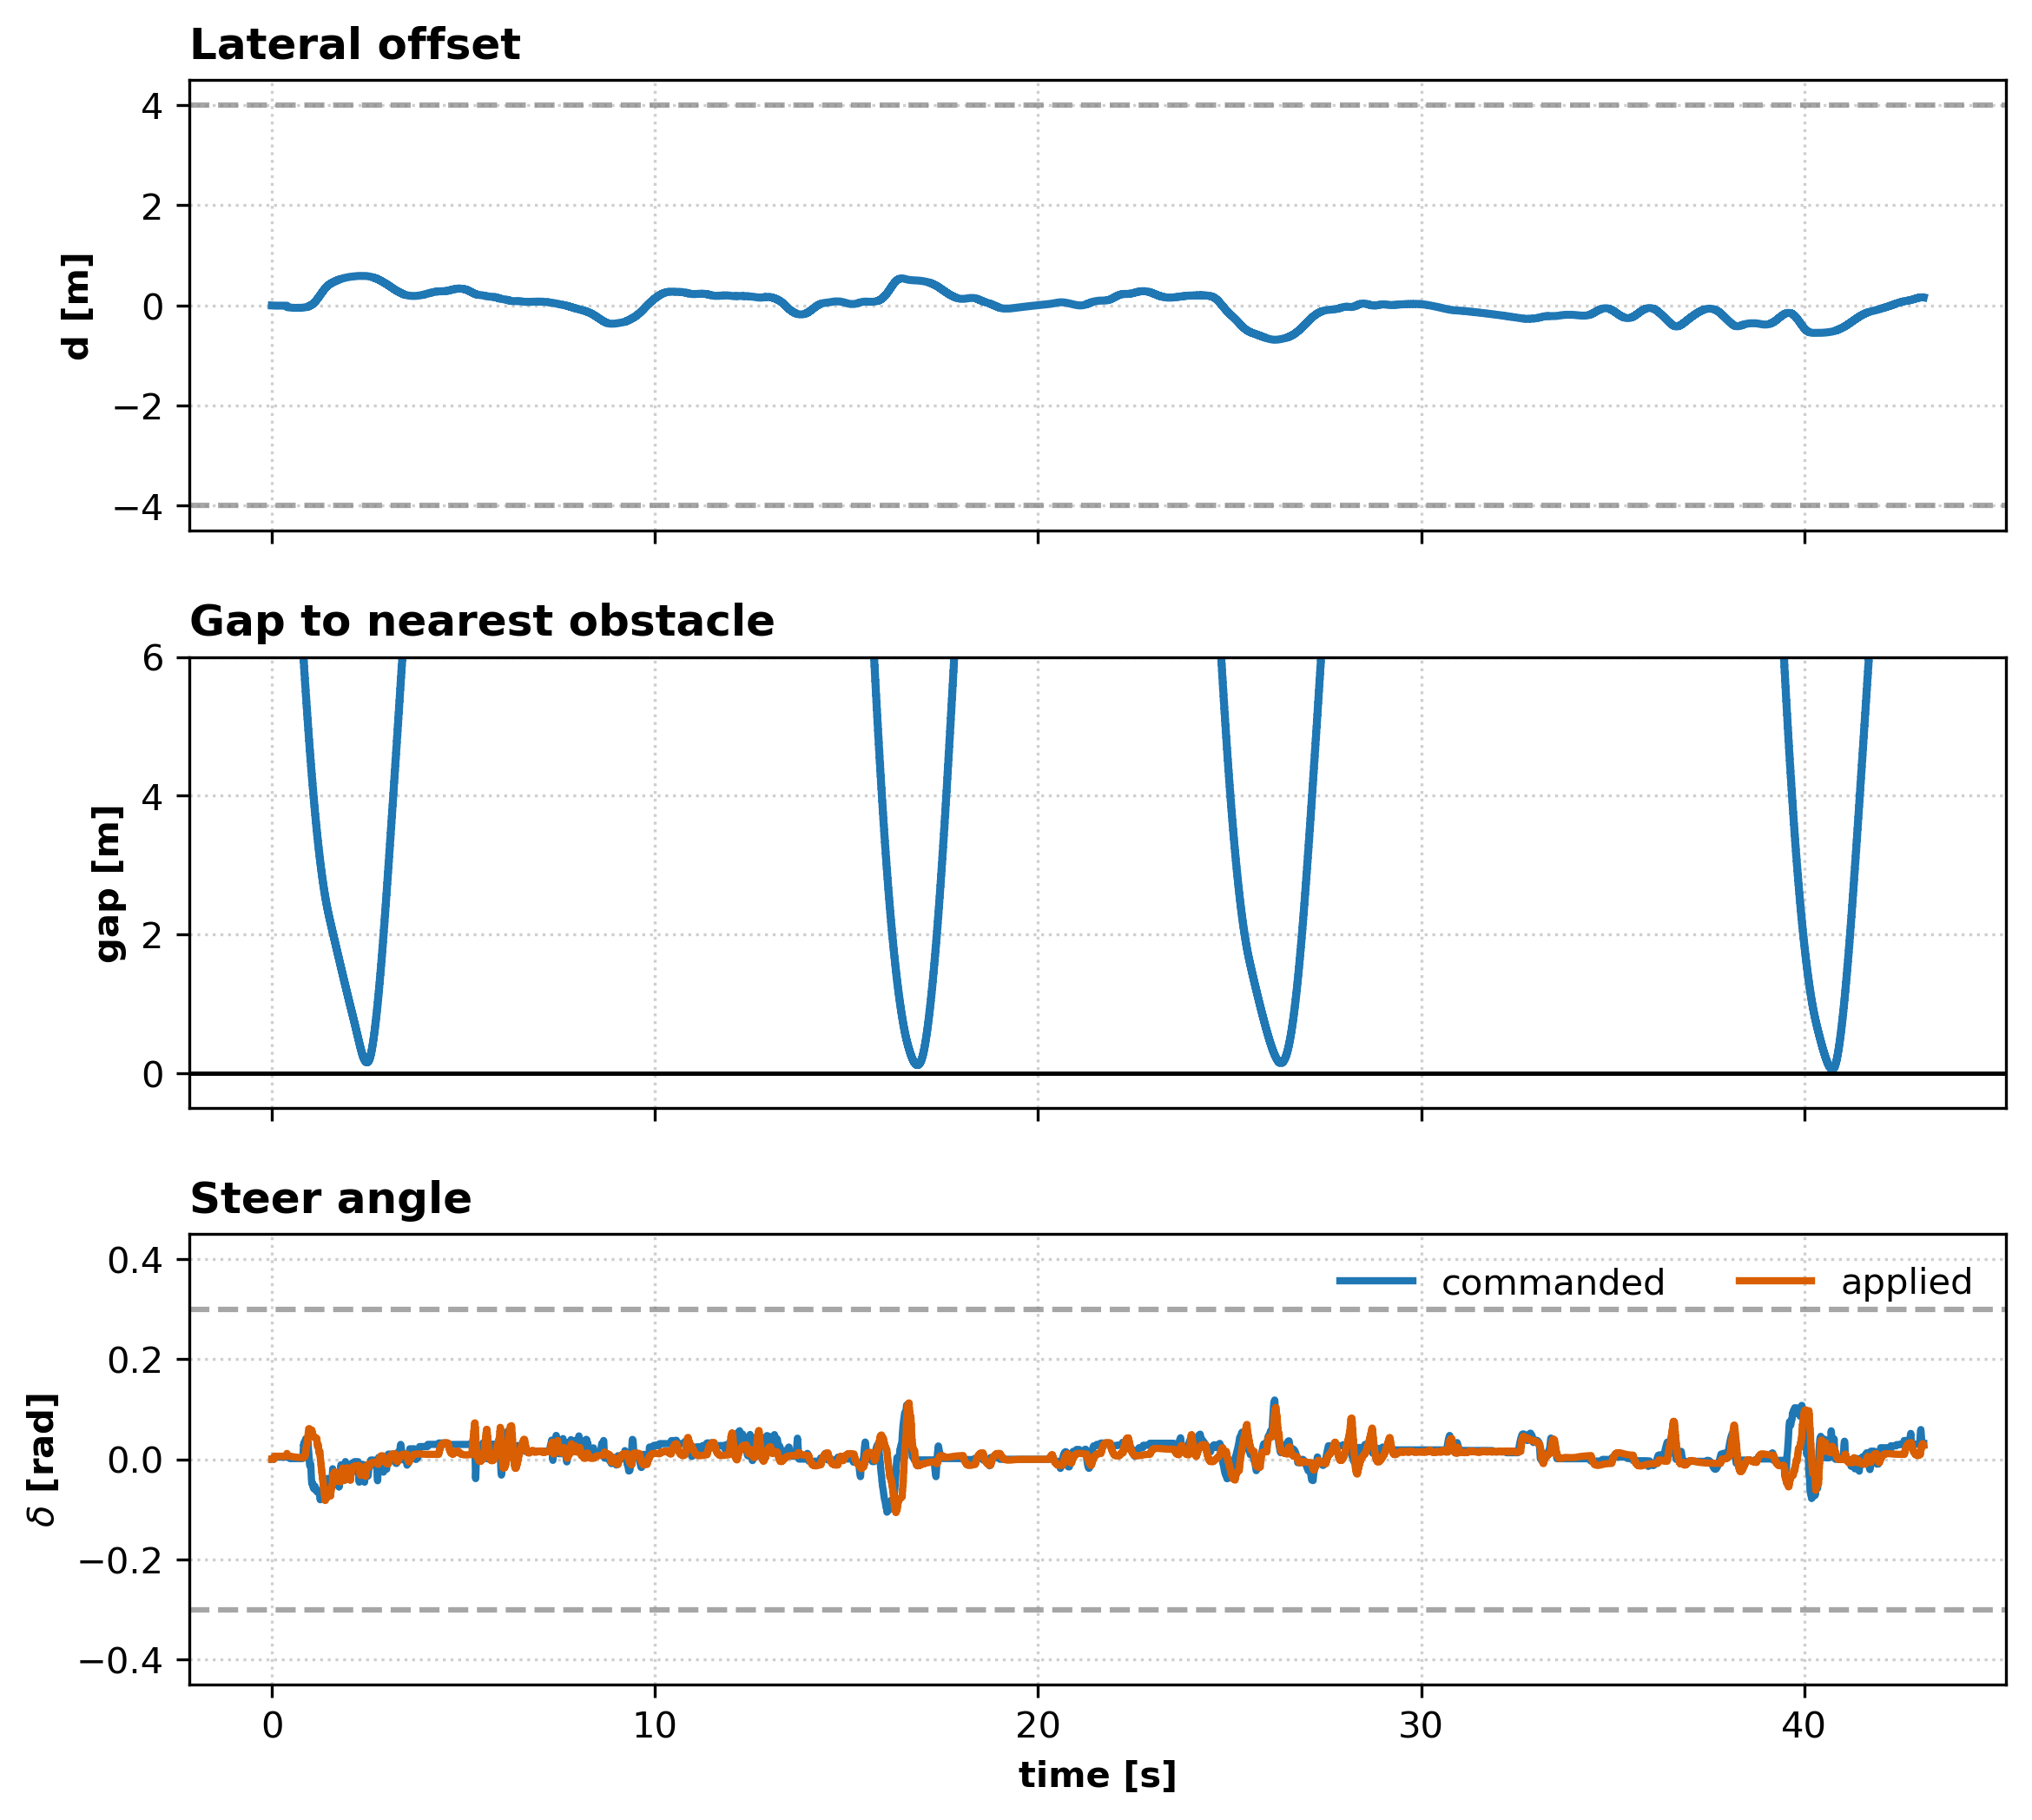
\includegraphics[width=.73\textwidth]{figures/slalom_y_response.png}
\caption{Recorded slalom simulation output from \cite{mulakaloori2026repo}: top, lateral centerline offset $d(t)$, used here as the lateral $y$ response; middle, estimated obstacle gap; bottom, commanded and inferred applied steering. Reproduced from the repository's \texttt{results/bag\_slalom\_benchmark.png} (Apache-2.0). The 4~m dashed lines are source-plot guides.}
\label{fig:yresponse}
\end{figure*}

\subsection{New Simplified Circuit Run}
To assess whether the same implementation can follow a different centerline, we constructed an original closed circuit inspired by the broad layout of Yas Marina. This is neither a scaled copy nor an official circuit map. A periodic spline through manually selected points generated both the occupancy map and the controller centerline. The resulting 322.20~m route has a 2.9~m road width, a minimum sampled radius of approximately 3.98~m, and a map resolution of 0.06~m/pixel. We used the RTX~3050 laptop GPU in this study, the same 100-stage, 5,000-sample controller, and a reduced maximum commanded speed of 7.0~m/s. No extra obstacles were added. The map generator, launch configuration, ROS~2 bag, and analysis script are included in the accompanying \texttt{RMPC\_F1TENTH} project folder.

The 161.36~s local recording contains two detected laps, of 63.70 and 59.41~s. Figure~\ref{fig:localf1} plots all 40,312 recorded odometry samples against the generated centerline, together with $d(t)$ calculated using the same nearest-sample normal projection as the repository evaluator. The maximum recorded $|d|$ is 0.662~m, below the 1.45~m centerline-to-map-edge distance. This geometric observation does not by itself certify full vehicle-body clearance. The local 99th-percentile \texttt{/drive} message interval is 6.82~ms, and its maximum is 17.93~ms; neither value isolates solver execution. Since the circuit length, curvature, speed cap, and computer differ from the source IMS experiments, their lap times should not be treated as a matched performance comparison.

\begin{figure*}[t]
\centering
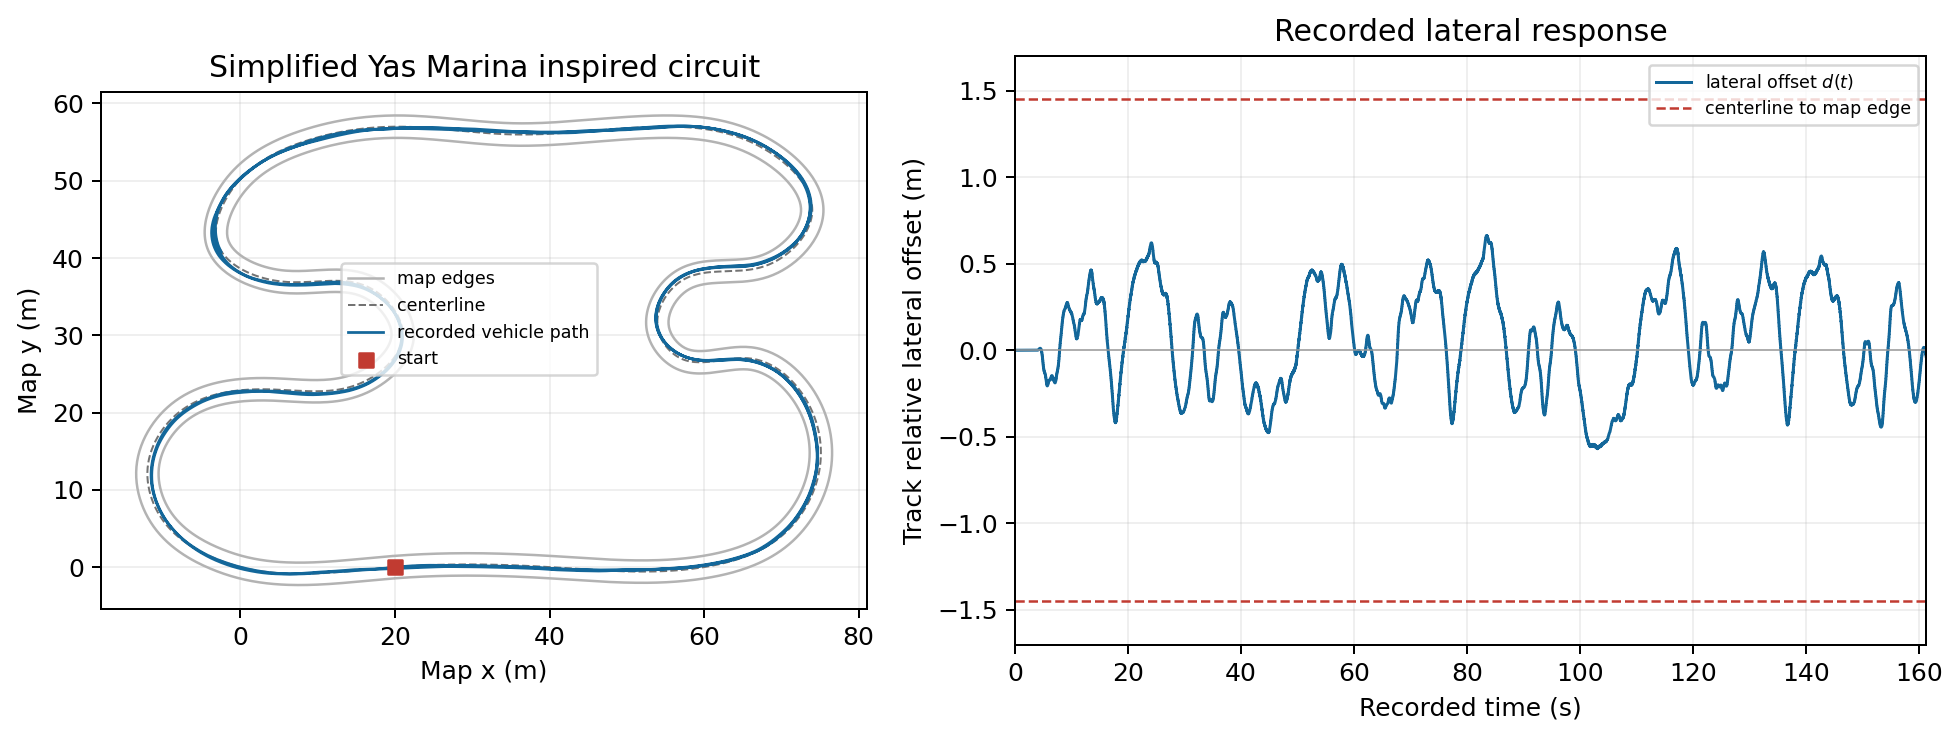
\includegraphics[width=.95\textwidth]{figures/local_f1_track_response.png}
\caption{New local run on the original simplified Yas-Marina-inspired map. Left: generated map edges and centerline with the recorded vehicle path. Right: track-relative lateral response $d(t)$, the requested lateral simulation $y$ variable. Red dashed lines mark the 1.45~m centerline-to-map-edge distance, not a body-clearance bound. The trace is computed from the archived ROS~2 bag.}
\label{fig:localf1}
\end{figure*}

\subsection{Timing and Interpretation}
The saved 99th-percentile \texttt{/drive} intervals are below 20~ms in both runs, but the slalom maximum is 335.87~ms. The repository suggests a startup transient, without a timestamp-level analysis to verify that explanation. We therefore do not claim that every cycle met a 20~ms deadline. The observed intervals also cannot be compared directly with the approximately 3~ms GPU computation and 100~Hz control rate reported for the distinct full-scale vehicle and hardware in \cite{muraleedharan2025racing}. The repository's single-run results show an operating F1TENTH control pipeline and a positive estimated slalom margin, while leaving repeatability, exact deadline satisfaction, and robustness to new obstacle layouts open.

\section{Controlled Comparison and Sensitivity Study}
\subsection{Experimental Protocol}
To compare steering methods with a common speed policy, we extended the local F1TENTH controller with a Pure Pursuit branch \cite{coulter1992pursuit}. Its target is interpolated 1.5~m ahead in centerline arc length and its steering law is
\begin{equation}
\delta_{\mathrm{PP}}=\operatorname{atan2}\!\left(\frac{2L y_g}{x_g^2+y_g^2},1\right),
\end{equation}
where $(x_g,y_g)$ is the target in the vehicle frame and $L=0.3302$~m. Both branches use the same curvature- and forward-distance-based speed command, a 7.0~m/s speed ceiling, $\pm0.4189$~rad steering limit, and 3.2~rad/s steering slew limit. This isolates the steering choice more closely than comparing two independently tuned speed planners; it does not test a globally optimized racing policy. The RMPC branch retains its original weights, 100-stage horizon, 20~ms prediction step and seven basis coefficients. We varied only the number of sampled trajectories: 1,000, 2,500 and 5,000.

The test harness calls the actual compiled C++/CUDA controller through a synchronous stream. It passes the current ground-truth vehicle state and 819-beam LiDAR scan, waits for one steering/speed command, then advances F1TENTH Gym by two 10~ms RK4 physics steps. Thus the control period is exactly 20~ms in simulation time, independent of wall-clock execution. This design measures computational cost without ROS transport, GUI rendering or simulator time in the timed region. A monotonic timer encloses the synchronized RMPC \texttt{solve()} call, including GPU sampling, rollout, transfers and host-side selection; it is not GPU-kernel-only time. A second timer covers perception, controller callback and publication. The first simulated second is omitted from steady timing summaries, while all states remain in the lap and tracking metrics. These computation times should not be conflated with the earlier asynchronous ROS \texttt{/drive} intervals.

We ran ten independent restarts per method and map, with paired seeds 81000--81009 and randomized run order: 80 nominal trials. Each trial starts near centerline point 0 from rest, with lateral perturbation $\mathcal N(0,0.05^2)$~m clipped to $\pm0.12$~m and yaw perturbation $\mathcal N(0,0.01^2)$~rad clipped to $\pm0.03$~rad. LiDAR range noise has 0.01~m standard deviation; ground-truth odometry is supplied. Each run ends on a Gym collision, completion of one unwrapped centerline length, or a 180~s simulated-time limit. Root-mean-square (RMS) $d$ uses all state samples in the trial. Lap time is reported only after completion. A separate repeat of the pilot seed reproduced the state and command sequence exactly; pilot seed 70001 was excluded from the study.

The simulator's nominal F1TENTH body has mass 3.74~kg, friction coefficient 1.0489 and width 0.31~m. The inherited RMPC prediction model uses 3.47~kg, 0.523 and 0.2032~m; these model differences are retained. The archived controller YAML, simulator settings, map and centerline hashes, source-script and binary hashes, per-step traces, run order and numerical summaries are in the accompanying \texttt{RMPC\_F1TENTH/experiments} folder. The controlled traces are \texttt{NPZ} arrays; the earlier ROS~2 bags are a separate dataset.

\subsection{Nominal Results and Sample Count}
All 80 nominal trials completed one lap without a Gym collision. Table~\ref{tab:controlled} reports the ten-trial mean and sample standard deviation, and Fig.~\ref{fig:controlled} shows each trial. On both maps, the selected Pure Pursuit baseline has lower RMS centerline error and mean lap time than the 5,000-sample RMPC under the shared speed policy. Pairing by seed, RMPC minus Pure Pursuit RMS error averages 0.142~m on IMS (95\% paired bootstrap interval 0.128--0.156~m) and 0.213~m on the new circuit (0.201--0.223~m). Corresponding paired lap-time differences are 3.68~s (2.42--4.86~s) and 2.23~s (1.11--3.49~s). These bootstrap intervals resample ten seed pairs 10,000 times; they describe uncertainty under the narrow perturbation protocol, not general controller ranking. A 10/10 completion count does not imply a zero failure probability on unseen tracks.

\begin{table*}[t]
\centering\small
\caption{Fixed 50 Hz study, ten independent trials per row. Means $\pm$ sample SD are over trials; lap time is reported for completed trials. P99 is calculated within each trial and then averaged.}
\label{tab:controlled}
\begin{tabular}{llrrrr}
\toprule
Track & Controller & Completed & Lap (s) & RMS $d$ (m) & Pipeline P99 (ms)\\
\midrule
IMS & Pure Pursuit & 10/10 & 49.83 $\pm$ 0.03 & 0.042 $\pm$ 0.001 & 0.144 $\pm$ 0.056 \\
IMS & RMPC 1000 & 10/10 & 55.04 $\pm$ 1.33 & 0.218 $\pm$ 0.015 & 1.267 $\pm$ 0.098 \\
IMS & RMPC 2500 & 10/10 & 55.98 $\pm$ 2.43 & 0.214 $\pm$ 0.033 & 1.256 $\pm$ 0.075 \\
IMS & RMPC 5000 & 10/10 & 53.51 $\pm$ 2.09 & 0.184 $\pm$ 0.024 & 1.308 $\pm$ 0.103 \\
New circuit & Pure Pursuit & 10/10 & 58.92 $\pm$ 0.05 & 0.056 $\pm$ 0.001 & 0.145 $\pm$ 0.057 \\
New circuit & RMPC 1000 & 10/10 & 62.62 $\pm$ 2.72 & 0.312 $\pm$ 0.033 & 1.288 $\pm$ 0.137 \\
New circuit & RMPC 2500 & 10/10 & 61.22 $\pm$ 1.62 & 0.278 $\pm$ 0.019 & 1.265 $\pm$ 0.101 \\
New circuit & RMPC 5000 & 10/10 & 61.16 $\pm$ 2.01 & 0.269 $\pm$ 0.018 & 1.266 $\pm$ 0.101 \\
\bottomrule
\end{tabular}
\end{table*}


\begin{figure*}[t]
\centering
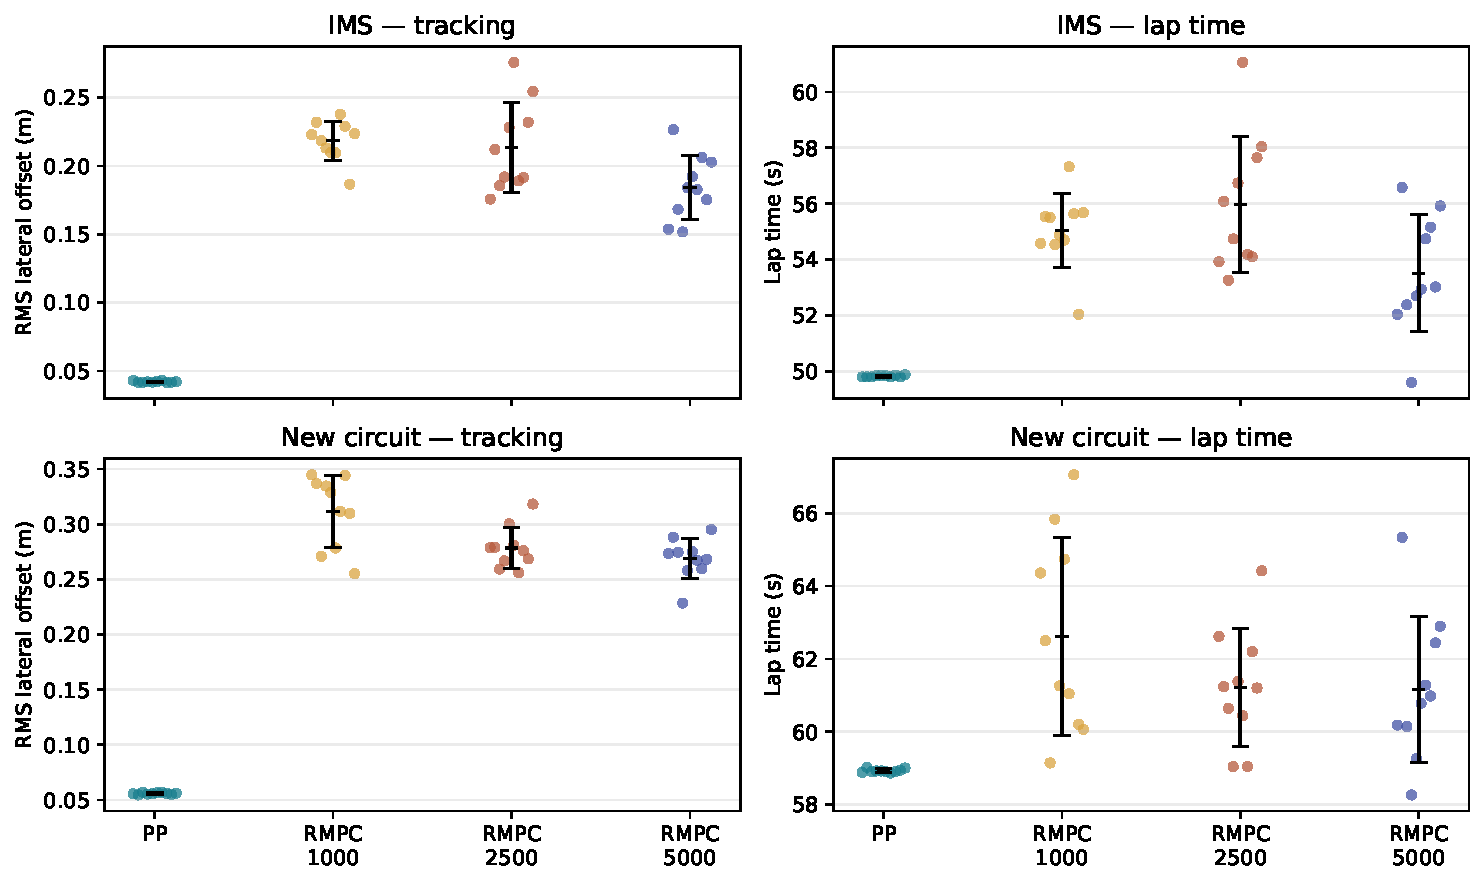
\includegraphics[width=.88\textwidth]{figures/controlled_comparison.pdf}
\caption{Ten independent nominal trials per condition. Dots are trial outcomes; black bars are mean and sample standard deviation. PP denotes Pure Pursuit. All 80 runs completed; the figure retains every lap and RMS offset.}
\label{fig:controlled}
\end{figure*}

Figure~\ref{fig:samples} shows that increasing RMPC samples from 1,000 to 5,000 changed the mean median synchronized solve-call duration only modestly: 0.881 to 0.919~ms on IMS and 0.886 to 0.919~ms on the new circuit. Mean RMS offset declined from 0.218 to 0.184~m on IMS and 0.312 to 0.269~m on the new circuit, but the 2,500-sample trial outcomes and lap times were not monotonic. Fixed transfer, synchronization and selection costs contribute to the measured call duration. Across all 100 controlled trials, the largest individual RMPC solve call was 5.72~ms. No observed solve call exceeded 20~ms in this unloaded synchronous harness; that fact alone does not establish an asynchronous ROS deadline guarantee.

\begin{figure*}[t]
\centering
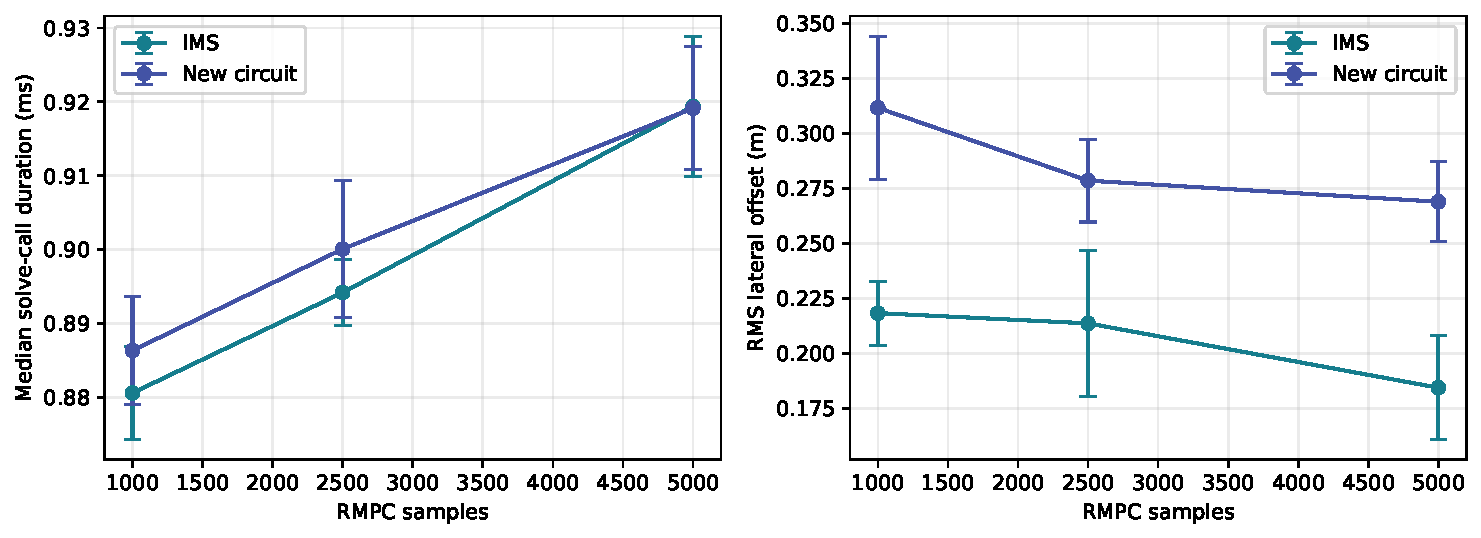
\includegraphics[width=.83\textwidth]{figures/sample_tradeoff.pdf}
\caption{RMPC sample-count sensitivity. Points are ten-trial means; bars show sample standard deviation across trial-level median solve durations (left) and RMS lateral errors (right). The timed solve call includes synchronized GPU work and CPU selection.}
\label{fig:samples}
\end{figure*}

\subsection{Unannounced Low-Grip Sector}
For a separate robustness probe, we repeated the new-circuit comparison at 5,000 RMPC samples with the same ten paired seeds. The simulator's friction coefficient drops from 1.0489 to 0.35 between 15\% and 35\% of centerline progress, then returns to 1.0489. Neither controller is informed of the change; RMPC's assumed coefficient stays at 0.523. All 20 runs completed without a Gym collision or center crossing beyond the nominal map half-width. Mean RMS $d$ rose from 0.056 to 0.145~m for Pure Pursuit and from 0.269 to 0.334~m for RMPC. Mean laps changed from 58.92 to 59.19~s and from 61.16 to 61.75~s, respectively. Figure~\ref{fig:slippery} shows the preselected seed 81000, with the affected sector shaded. The sector models an abrupt parameter change; it does not model water, changing tire temperature or sensor delay. The absence of failures in ten trials per method is limited evidence of robustness.

\begin{figure*}[t]
\centering
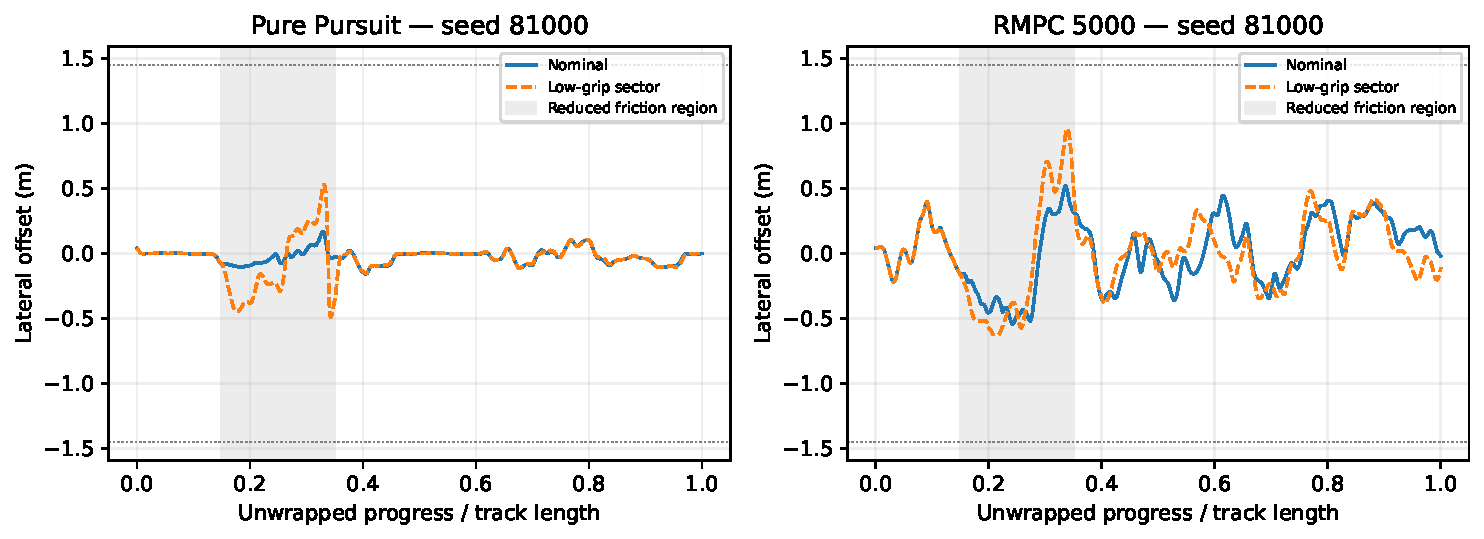
\includegraphics[width=.83\textwidth]{figures/slippery_response.pdf}
\caption{Nominal and reduced-grip lateral responses for the predetermined seed 81000. The shaded interval is the simulator's low-grip sector ($\mu=0.35$). Dotted lines show the new circuit's 1.45~m centerline-to-map-edge distance, not full-body clearance.}
\label{fig:slippery}
\end{figure*}


\section{Discussion}
The full-scale reference study and the F1TENTH case share a randomized predictive-control idea, but their control problems differ in important ways. The full-scale controller addresses simultaneous lateral and longitudinal inputs while tracking a speed-bearing race line and operating near estimated tire-force constraints \cite{muraleedharan2025racing}. The F1TENTH implementation uses a centerline, optimizes steering against local costs, and then calculates a separate speed command. Its obstacle handling uses an inflated local occupancy grid and a forward-distance speed heuristic. A comparison of their lap times or GPU timings would therefore mix hardware, vehicle scale, track geometry, controller scope, and measurement method.

The $d(t)$ signal in Fig.~\ref{fig:yresponse} is useful because it shows how a lateral tracking variable evolves during obstacle passages. However, a small $|d|$ alone does not prove that the vehicle stayed within track limits: safe lateral position depends on local left and right widths, body dimensions, and obstacle occupancy. Similarly, the positive 0.054~m reported obstacle gap is a minimum over a simplified circle model, not a robust safety margin. The near-zero clearance warrants more detailed review of the underlying trajectory if those bags become available.

The timing record also illustrates why several quantities must be kept separate. The 20~ms value is a configured rollout step. The 16.79~ms slalom P99 is a distributional property of message spacing. The 335.87~ms maximum is a recorded outlier whose cause has not been confirmed. None is an isolated GPU solve measurement. An instrumented study should log solver start and finish times, callback timestamps, and message publication times on the same clock, then report deadline misses directly.

The new controlled study supplies a matched steering baseline and repeated trials for two maps. Its narrower speed cap, synchronous stepping, and different hardware prevent direct numerical comparison with the repository's ROS~2 bags. Further work should vary obstacles, speed profiles, sensor delay, vehicle parameters and maps, with controller tuning fixed on separate development seeds.

\section{Limitations and Conclusion}
The original IMS evidence is limited to two saved run summaries and plots; their raw bags are unavailable. The new circuit ROS~2 bag represents one asynchronous run with two laps. The separate controlled dataset has ten independent trials per condition, but only two maps, small initial perturbations, ground-truth odometry, one fixed Pure Pursuit lookahead, one speed cap and a simplified friction transition. Its results are sensitive to these choices. The slalom obstacle-margin calculation uses three fixed points and circular radii, so it does not certify contact-free driving under a full vehicle footprint. The repository itself notes that obstacle-avoidance runs may become unstable after several runs \cite{mulakaloori2026repo}. The controlled-study times exclude ROS transport and the simulator; they establish computation cost in this harness, not a deployed deadline guarantee.

This JAMRIS case study connects the full-scale RMPC formulation to the F1TENTH implementation while preserving their differences. The source slalom plot and the new circuit recording show the lateral $d(t)$, or track-relative $y$, response. In the additional controlled trials, both algorithms completed all laps, while Pure Pursuit achieved lower mean tracking error and faster mean laps under the matched speed policy. Increasing RMPC samples produced small, variable changes in tracking and solve time. The archived traces and configurations make these bounded findings reproducible and provide a basis for a stronger obstacle-aware comparison.

\AuthorNote
\raggedend
\bibliographystyle{jamris}
\bibliography{references}
\end{document}
